\subsection{Матожидание}

    \comment{параметричесикй интервал выживаемости при увеличении шума уменьшается}

    На графике \ref{EV_cyclic} видно, что 

    Перейдем к рассмотрению графика \ref{EV_cyclic} усредненных значений математического ожидния, полученных из нескольких экспериментов. 
        
    \begin{figure}
        \centering
        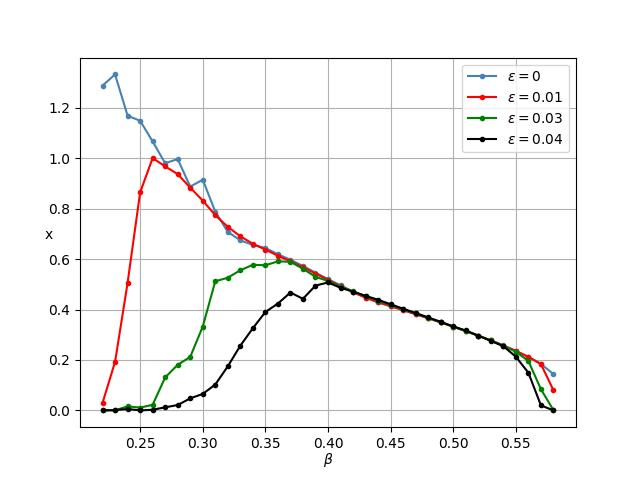
\includegraphics[width=\textwidth]{stochastic/images/EV_cyclic.jpg}
        
        \captionsetup{justification=centering}
        \caption{Матожидание}
        \label{EV_cyclic}
    \end{figure}

    На графике матожидания видно, что значения бифуркации при уменьшении параметра \(\beta\) растет, доходит до какого-то значения и сваливается в ноль. Заметим также, что при увеличении интенсивности наша модель начинает уходить в ноль при более больших значениях параметра \(\beta\). Это связано с тем, что при более высокой интенсивноти, шум оказывает более сильное влияние на развитие популяции.

    \comment{При чем, если есть шум, то уходим в ноль всегда, а при остуствии шума начинается зона хаоса}

    \comment{Точка начала сваливания в ноль обусловлена траекториями...}

    \comment{Теперь про касания...}

    \comment{А разные шумы?}